\section{Theoretische Grundlagen}
\subsection{Doppelbrechung}
Doppelbrechung ist eine Eigenschaft von optisch anisotropen Stoffen. In diesen ist die Ausbreitungsgeschwindigkeit abhängig von Richtung und Polarisation der durchdringenden Welle. Das führt dazu, dass die Welle in zwei Teilstrahlen aufgespalten wird.


\subsection{Pockels Effekt}
Der Pockels Effekt tritt nur in Kristallen ohne Symmetriezentren auf: Doppelbrechung wird durch Anlegen einer externen Spannung erreicht.
Die Begründung dafür is, dass die Permittität $\epsilon$ nicht konstant ist, sondern vom angelegten elektrischen Feld abhängig ist. 
Die Permittität ist definiert über $\epsilon = \frac{\d D}{\d E}$ wobei $D$ definiert ist wie folgt: 
\begin{equation}
D = aE +bE^2+cE^3+... \qquad \textrm{mit } a,b,c = const
\end{equation}
Daraus folgt
\begin{equation}\label{epsilon}
\epsilon = a + 2bE + 3cE^2 + ...
\end{equation}.\par
Der Brechungsindex $n$ ist abhängig von $\epsilon$, sodass eine Änderung des Magnetfeldes eine Änderung im Indexellypsoid hervorruft. Dies ist der elektrooptische Pockels Effekt. Hier ist vor allem der lineare Term von \ref{epsilon} ausschlaggebend.
\subsection{Aufbau der Pockels Zelle}
Die im Versuch verwendete Pockels Zelle besteht aus 4 Ammoniumdihydrogenphosphat (ADP, $NH_4H_4PO_4$) Kristallen, welche im $45^\circ$-Y-Cut vorliegen.\\
Der Indexellipsoid  des Kristalls bis zu ersten Ordnung ist wie folgt:
\begin{equation}
	\frac{x_1^2}{n_1^2} + 2 r_{41} x_2 E_1 x_3 + \frac{x_2^2}{n_1^2}+ 2 r_{41} x_1 E_2 x_3 + \frac{x_3^2}{n_3^2} +  2 r_{63} x_1 x_2 E_3 = 1
\end{equation}

Hierbei ist optische Achse im feldfreien Fall die $x_3$ Achse. 	Wenn ein Elektrisches Feld entlang der $x_1$ Achse angelegt ist, gilt das Folgende:
\begin{equation}
		\frac{x_1^2}{n_1^2} + 2 R_{41} x_2 E_1 x_3 + \frac{x_2^2}{n_1^2}+  \frac{x_3^2}{n_3^2} = 1
\end{equation}

Y-Cut: Koordinatenwechsel durch Drehung con $45^\circ$ um $x_1$ Achse:
\begin{equation}
	x_2 = \frac{1}{\sqrt{2}} \left(x_2^\prime x_3^\prime \right) \qquad
	x_3 = \frac{1}{\sqrt{2}} \left(x_2^\prime x_3^\prime \right) 
\end{equation}
Nach der Herleitung in der Versuchsanleitung \cite{anleitung} folgt nun für dem Brechungsindex der jeweiligen Polarisationskomponenten bei Lichteinfall der $x_2^\prime$ ($x_3^\prime$) Richtung 
\begin{equation}
n_{x_2^\prime} = \frac{n_x}{\sqrt{1+ r_{41}E_1 n_x^2}} \approx n_x + \frac{1}{2}r_{41}E_1 n_x^3
\end{equation}
In einem Kristall der Länge $l$ lautet die Phasenverschiebung nun
\begin{equation}
\omega t = \frac{2\pi}{\lambda}\left(n_1 - n_{x_2^\prime}\right)
\end{equation}
Weil die optische Achse und der k-Vektor in einem Winkel von $45^\circ$ zueinander stehen, trennt sich der eingehende Lichtstrahl in einen ordentlichen und außerordentlichen Strahl, welche durch einen zweiten ADP Kristall, der um $180^\circ$ zum ersten verdreht ist. So werden die strahlen wieder vereinigt. Ihre Phasenverschiebung aufgrund der unterschiedlichen Ausbreitungsgeschwindigkeiten ist nun 
\begin{equation}
\omega t = \frac{2\pi}{\lambda}\cdot2\cdot\left(n_1 - n_{x_2^\prime}\right)
\end{equation}

Es ist zusätzlich noch die Natürliche Doppelbrechung vorhanden, welche um ein weiteres Kristallpaar mit Winkel $90^\circ$ verbaut ist. Dass der Pockels Effekt nicht gleichzeitig kompensiert wird, wurde das Elektrische Feld an diesen umgekehrt. Dieser Aufbau mit Strahlengang ist in Abbildung \ref{kristalle} erkennbar. Die resultierende Phasenverschiebung ist somit 
\begin{equation}
\omega t = \frac{4\pi}{\lambda}r_{41} E_1 n_x^3 l
\end{equation}
Bei einer Phasenverschiebung um $\pi$ und einem Elektrischen Feld von $E= \frac{U}{d}$ gilt somit:
\begin{equation}
\label{pockelsgleichung}
r_{41} = \frac{\lambda d}{4 l U_{\lambda/2}} \sqrt{\frac{1}{2}\left(\frac{1}{n_1^2}+\frac{1}{n_3^2}\right)}^3
\end{equation}

\begin{figure}[h]
	\centering
	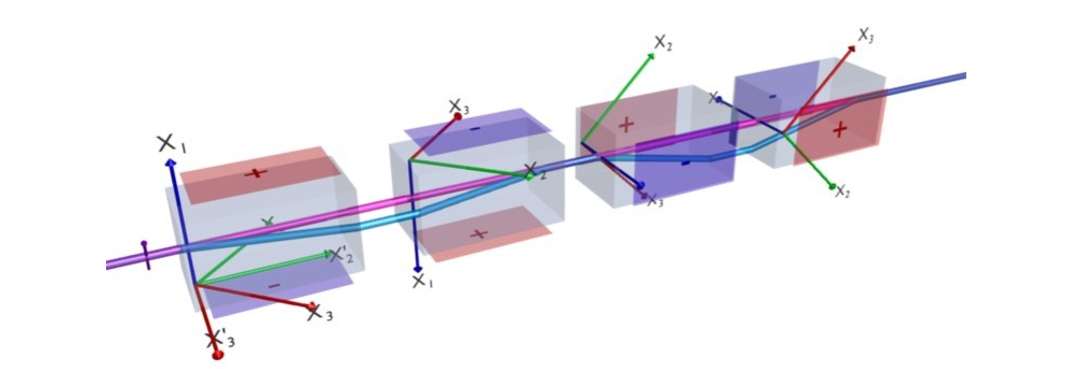
\includegraphics[scale=0.7]{Bilder/kristalle}
	\caption[Aufbau der Pockels Zelle]{\small Das Bild zeigt den Aufbau der verwendeten Pockels Zelle. Die Elektroden für den Aufbau der elektrischen Felder sowie die Strahlenverläufe sind auch eingezeichnet.}
	\label{kristalle}
\end{figure}


\subsection{Faraday Effekt}
Der Faraday Effekt ist eine Magnetfeldinduzierte Doppelbrechung, auch Magnetooptischer Effekt genannt. Er erfolgt in isotropen Medien bei Anlegung eines Magnetfeldes parallel zur Ausbreitungsrichtung des Lichts. Das linear polarisierte eingehende licht kann in zwei entgegengesetzt drehende zirkularpolarisierte Wellen aufgespalten werden. Die Links- und Rechtsdrehenden zirkularpolarisierten Teilwellen können das Medium bei angelegtem Magnetfeld nicht gleich schnell durchqueren. Dies führt bei verlassen des Mediums zu einer Phasenverschiebung der linear polarisierten Kombination der beiden zirkularpolarisierten Wellen. Dieser Drehwinkel $\alpha$ kann über die Nachfolgende Formel aus der Magnetischen Feldstärke $H$, der Länge des Mediums $l$ und der Verdetkonstante $V$, welche materialabhängig ist, bestimmt werden. 
\begin{equation}\label{faraday_unfertig}
\alpha = V \cdot l \cdot H
\end{equation}
\subsection{Magnetfeld einer realen Spule}
Für die Berechnung des Magnetfeldes einer realen Spule wird das Biot-Savart'sche Gesetz verwendet. Es ist definiert als 
\begin{equation}
\label{biot-savart}
d B = \frac{\mu_0}{4 \pi} I d \vec{l} \times \frac{\vec{r}-\vec{r^\prime}}{\left|\vec{r}-\vec{r^\prime}\right|^3}
\end{equation}
Nach der Herleitung im Staatsexamen von B.Herrmann \cite{staatsex_farpock}, erhält man für das Magnetfeld der realen Spule nach Integration über Länge und Dicke den nachfolgenden Ausdruck:
\begin{equation}
H(z) = \frac{N I}{2L(x_2-x_1)}\left[
(L-z) \ln\left(\frac{x_2 + \sqrt{(L-z)^2+x_2^2}}{x_1 + \sqrt{(L-z)^2+x_1^2}}\right) + z \ln \left(\sqrt{\frac{x_2 + \sqrt{z^2 +x_2^2}}{x_1 + \sqrt{z^2 +x_1^2}}}\right) 
\right]
\label{realFormel}
\end{equation}
Hierbei sind $x_1$ der innerer Spulenradius, $x_2$ der äußere und $L$ die Länge der Spule. Bei einsetzen der Parameter folgt nach \cite{staatsex_farpock} für die Gleichung \ref{faraday_unfertig}: 
\begin{equation}
\alpha = V \cdot 2556 \cdot I 
\label{r41}
\end{equation}